\pagebreak
\section{$e$-Funktion}\label{sec:e-Funktion}
Die E-Funktion ist einen Unterart der Exponentialfunktion (\ref{sec:Exponentialfunktionen}) sie hat, anders als eine Exponentialfunktion, einen belibige Zahl als Basis. Die Basis einer $e$-Funktion ist die eulischere Zahl $e$. 
\subsection{Entstehung von $e$} \label{sec:E-Funktion/Entstehung von e}
Die Entstehung von $e$ ist ein Grenzwertprozess...
%ToDo Entstehung von e

\subsection{Normalform}\label{sec:E-Funktion/Normalform}
Die Normalform einer $e$-Funktion lautet
\[a\cdot e^{k\cdot x}\]
%TODO Normalform der e-Funktion hinzufügen

\subsection{Ableiten der $e$ Funktion}\label{sec:E-Funktion/Ableiten der e Funktion}
Die besonderheit bei $e$-Funktionen ist, dass die Differenzierte und Integrierte Funktion jeweils immer gleich ist. 
%ToDo Hier fehlen Informationen über das Integrieren und Differenzieren
\subsubsection{Faktorregel}\label{sec:E-Funktion/Normalform} 
Ähnlich wie bei dem normalen Ableiten bei einer ganzrationalen Funktion lässt sich hier die Faktorregel anwenden.
%ToDo Hier fehlen Informationen bezüglich des Ableitens und Differenzieren
\subsubsection{Kettenregel}
Liegt eine verkette Funktion vor, so kann diese mithilfe der Kettenregel abgleitet werden. Bei einer verketteten Funktion gibt es eine äußere Funktion und eine innere Funktion. 
Die Kettenregel ist ein wichtiges Hilfsmittel beim Ableiten von komplexeren Funktion, die sich in eine innere und äußere Funktion einteilen lassen. Die Kettenregel lautet wie folgt.
\begin{align*}
	f(x)&=u(v(x))\\
	f'(x)&=u'(v(x))\cdot v'(x)
\end{align*}
Wobei $u(x)$ die äußere Funktion darstellt und $v(x)$ die äußere Funktion. 
Um mit der Kettenregel zu integrieren wendet man folgende Normalform an. 
\begin{align*}
	f(x)=u(v(x))\\
	F(x)=\frac{U(v(x))}{v'(x)}
\end{align*}
\begin{beispiel}
	\begin{align*}
		f_1(x)=e^{\frac{1}{2}x}\tag{Aufteilen in innere- und äußere Funktion}\\
		v(x)=\frac{1}{2}x \tag{Die innere Funktion}\\
		u(x)=e^x\tag{Die äußere Funktion}\\
	\end{align*}
	Anschließend werden die Funktionen einzeln abgleitet und wieder mit der Form zusammen gebracht.
\end{beispiel}
\subsubsection{Produktregel}
Die Produktregel ist ein weitere Möglichkeit Funktionen, die mit einander multipliziert werden, zu berechnen.
\[f(x)=u(x)\cdot v(x)\]
\[f'(x)=u(x)\cdot v'(x)+u'(x)\cdot v(x)\]
\subsubsection{Differentialgleichungen}
Differentialgleichungen werden vorwiegend genutzt, um eine gesuchte Funktion mit einer Gleichung zu erhalten. Konkret bedeutet dies, dass eine Differentialgleichung 1. Ordnung
die Ausgangsfunktion und die Ableitung enthält. Allerdings bezieht sich dies nur auf e-Funktionen. So kann man beispielsweise eine e-Funktion wie folgt ableiten. 

\begin{beispiel}
	\begin{align*}
		f'(x)=k\cdot f(x)\\
	\end{align*}
In der Anwendung von Differnetialgleichungen gibt es außerdem noch die Möglichkeit Bedingungen aufzustellen ($f(0)=1$). Mit solchen Bedingungen kann man wie folgt umgehen.
\end{beispiel}

\begin{beispiel}
\begin{align*}
	f(0)=1\tag{Bedingung}\\
	f(0)=e^{k\cdot 1}\tag{Nach $k$ auflösen}\\
	ln(f(0))=k\cdot 1\tag{Dividieren durch 1}\\
	ln(f(0))=k\\
	\Rightarrow f'(x)=ln(f(0))\cdot f(x)
\end{align*}
\end{beispiel}

\subsection{$e$-Funktion aufstellen}
Um eine $e$-Funktion aufzustellen aus einem gegeben Sachverhalt, ist mindestens ein Wertepaar in der $(F;G)$ notwendig. Hierfür nimmt man zu Beginn die Normalform der $e$-Funktion ($ae^{kx}$)
\begin{align}
	f(x)&=ae^{kx}\\
	G&=ae^{kF}\\
	\frac{G}{a}&=e^{kF}\\
	ln\left(\frac{G}{a}\right)&=kF\\
	\frac{ln\left(\frac{G}{a}\right)}{F}&=k
\end{align}
\subsubsection{Erklärung}
Durch die Tatsache, dass ein Wertepaar gegeben ist und dies in die Form einer $e$-Funktion eingesetzt werden kann und somit für eine unbekannte Variable gesorgt wird, ist es möglich dies mithilfe des Logarithmus aufzulösen.
\begin{enumerate}
	\item Die Normalform der $e$-Funktion
	\item Das Wertepaar wird in die Normalform der $e$-Funktion eingesetzt
	\item Der Koeffizent wird durch Division auf die andere Seite gebracht. 
	\item Durch die Tatsache, dass der Logarithmus die Beziehung zwischen dem Ergebnis einer Potenzierung mit einem unbekannten Exponenten darstellt und $e$ in diesem Fall unsere Basis ist, dessen Exponenten genau die links neben dem Gleichheitszeichen ergibt. 
\end{enumerate}

\begin{beispiel}
	Gesucht ist die Funktion $f$. Diese soll mithilfe von der Normalform der $e$-Funktion aufgestellt werden. Der hierfür benötigte Punkt lautet $(5;12)$
	\begin{align*}
		f(x)&=ae^{kx}\\
		12&=e^{k5}\tag{Anwenden des ln}\\
		ln(12)&=k5\tag{Dividieren mit 5}\\
		\frac{ln(12)}{5}&=k\\
		f(x)&=e^{x\cdot \frac{ln(12)}{5}}
	\end{align*}
\end{beispiel}
\pagebreak
\subsection{Umformung von der normalen Exponentialfunktion zu der E-Funktion}\label{sec:E-Funktion/Umformung von der normalen Exponentialfunktion zu der E-Funktion}
Da sich die $e$-Funktion besonders gut differenzieren und integrieren lässt, nutzt man diese, um Sachverhalte darzustellen. Hierfür formt man die normale Exponentialfunktion so um, dass man sie als $e$-Funktion schreiben kann. Hierfür ist es relevant die Bedeutung der folgenden Normalform zu kennen. 
\subsubsection{Normalform}\label{sec:E-Funktion/Umformung von der normalen Exponentialfunktion zu der E-Funktion/Normalform}
\begin{align*}
	f(x)=a\cdot e^{k\cdot x+d}+c
\end{align*}
\geogebra{https://www.geogebra.org/m/bkar24wm}
\pagebreak
\subsubsection{$a$ - Streckfaktor}\label{sec:E-Funktion/Umformung von der normalen Exponentialfunktion zu der E-Funktion/Normalform/a - Streckfaktor}
Der Faktor $a$ ist bestimmt die Streckungs/Stauchungs des Graphen. Wird dieser negativ, so wird der Graph an der $X$-Achse gespiegelt. Der Grund hierfür ist, dass ist $a$ negativ, werden die gesamten Werte des Graphen ebenfalls negativ. 
%ToDo Hier fehlt ein Graph mit einem Vergleich
\begin{figure}[h]
\centering
	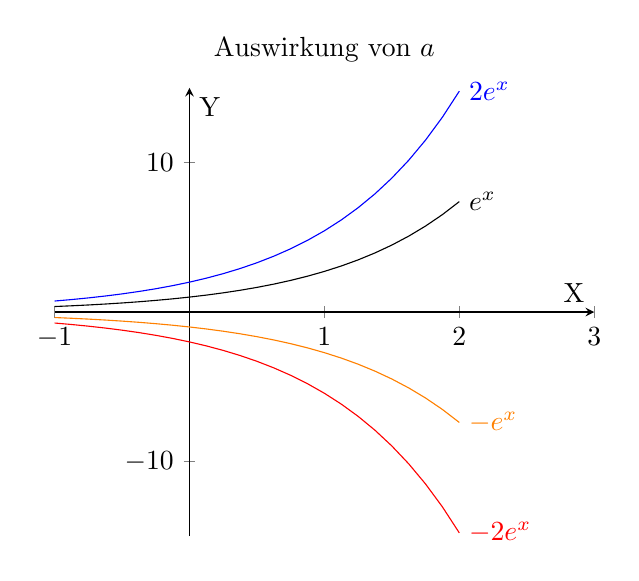
\begin{tikzpicture}
		\begin{axis}[
		title={Auswirkung von $a$},
		axis lines=middle,
		clip=false,
		xlabel={X},
		ylabel={Y},
		xmin=-1,
		xmax=3,
		ymin=-15,
		ymax=15
		]
		\addplot[domain=-1:2,blue]{2*exp(x)} node[right,pos=1]{$2e^x$};
		\addplot[domain=-1:2,black]{exp(x)}node[right,pos=1]{$e^x$};
		\addplot[domain=-1:2,orange]{-exp(x)}node[right,pos=1]{$-e^x$};
		\addplot[domain=-1:2,red]{-2*exp(x)}node[right,pos=1]{$-2e^x$};
		\end{axis}
	\end{tikzpicture}
	\caption{Auswirkung von $a$ auf den Graphen}
\end{figure}
\pagebreak
\subsubsection{$k$ - Koeffizent} \label{sec:e-Funktion/Umformung von der normalen Exponentialfunktion zu der E-Funktion/Normalform/k - Koeffizent}
Der Faktor $k$ ist ähnlich wie $a$ und bestimmt die Streckung und Stauchung des Graphen, allerdings wird der Graph an der $Y$-Achse gespiegelt, sobald dieser negativ wird. Dies wird begründet durch 
Die Begründung hierfür ist, dass wenn eine Zahl für $k$ eingesetzt wird, bestimmt $k$ wie oft $x$ multipliziert wird. Hierdurch erreicht der Graph schneller die selben $Y$-Wert für $k>0$. Ist $k<0$, so kehrt sich der Graph um aufgrund der Negätivität von $k$. Werden nun postive Werte für $x$ eingesetzt, so entstehen hierraus immernoch negative Zahlen, denn $-$ mal $+$ ergibt $-$. Somit werden die gleichen $Y$-Werte wie im Positiven erricht, jedoch im Negativen.
%ToDo Hier fehlt ein Graph mit einem Vergleich
\begin{figure}[h]
\centering
	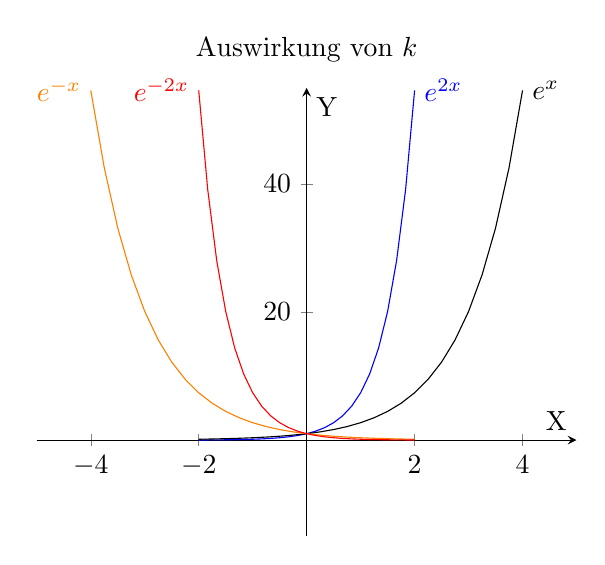
\begin{tikzpicture}
		\begin{axis}[
		title={Auswirkung von $k$},
		axis lines=middle,
		clip=false,
		xlabel={X},
		ylabel={Y},
		xmin=-5,
		xmax=5,
		ymin=-15,
		ymax=55
		]
		\addplot[domain=-2:2,blue]{exp(2*x)} node[right,pos=1]{$e^{2x}$};
		\addplot[domain=-2:4,black]{exp(1*x)}node[right,pos=1]{$e^x$};
		\addplot[domain=-4:2,orange]{exp(-1*x)}node[left,pos=0]{$e^{-x}$};
		\addplot[domain=-2:2,red]{exp(-2*x)}node[left,pos=0]{$e^{-2x}$};
		\end{axis}
	\end{tikzpicture}
	\caption{Auswirkung von $k$ auf den Graphen}
\end{figure}


\pagebreak
\subsubsection{$d$ - $X$-Achsenverschiebung}\label{sec:E-Funktion/Umformung von der normalen Exponentialfunktion zu der E-Funktion/Normalform/d - X-Achsenverschiebung}
Die Variable $d$ gibt die $X$-Achsenverschiebung an. Sei $d>0$ verschiebt sich der Graph nach links, andernfalls für $d<0$ verschiebt sich der Graph nach rechts. 
%ToDo Hier fehlt ein Graph mit einem Vergleich
\begin{figure}[h]
\centering
	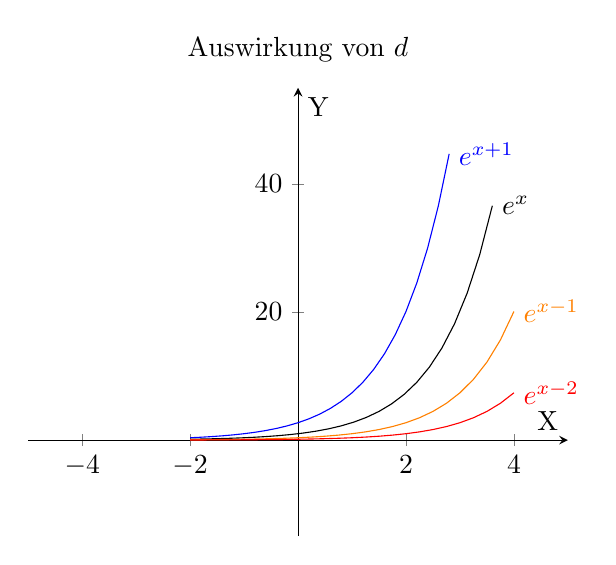
\begin{tikzpicture}
		\begin{axis}[
		title={Auswirkung von $d$},
		axis lines=middle,
		clip=false,
		xlabel={X},
		ylabel={Y},
		xmin=-5,
		xmax=5,
		ymin=-15,
		ymax=55
		]
		\addplot[domain=-2:2.8,blue]{exp(x+1)} node[right,pos=1]{$e^{x+1}$};
		\addplot[domain=-2:3.6,black]{exp(x)}node[right,pos=1]{$e^x$};
		\addplot[domain=-2:4,orange]{exp(x-1)}node[right,pos=1]{$e^{x-1}$};
		\addplot[domain=-2:4,red]{exp(x-2)}node[right,pos=1]{$e^{x-2}$};
		\end{axis}
	\end{tikzpicture}
	\caption{Auswirkung von $d$ auf den Graphen}
\end{figure}

\pagebreak
\subsubsection{$c$ - $Y$-Achsenverschiebung}\label{sec:e-Funktion/Umformung von der normalen Exponentialfunktion zu der E-Funktion/Normalform/c - Y-Achsenverschiebung}
Der Summand $c$ bestimmt die $Y$-Achsenverschiebung. Dies ist begründet durch die Tatsache, dass wenn ein Summand zu $x$ addiert wird, dieser immer um $c$ nach oben verschoben ist. 
\begin{figure}[h]
\centering
	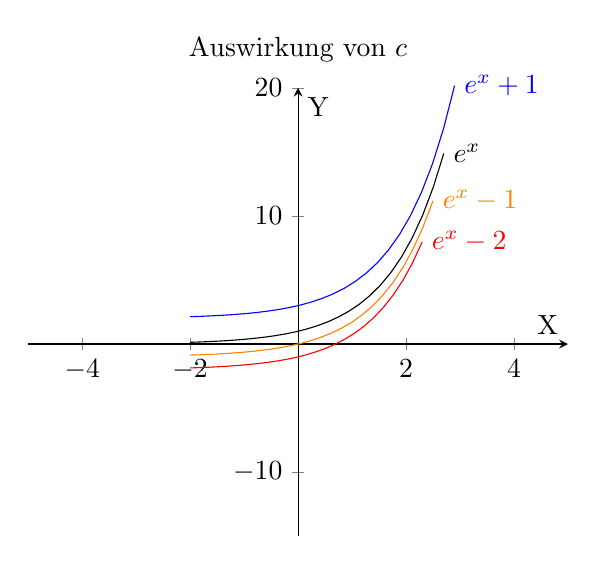
\begin{tikzpicture}
		\begin{axis}[
		title={Auswirkung von $c$},
		axis lines=middle,
		clip=false,
		xlabel={X},
		ylabel={Y},
		xmin=-5,
		xmax=5,
		ymin=-15,
		ymax=20
		]
		\addplot[domain=-2:2.9,blue]{exp(x)+2} node[right,pos=1]{$e^{x}+1$};
		\addplot[domain=-2:2.7,black]{exp(x)}node[right,pos=1]{$e^x$};
		\addplot[domain=-2:2.5,orange]{exp(x)-1}node[right,pos=1]{$e^{x}-1$};
		\addplot[domain=-2:2.3,red]{exp(x)-2}node[right,pos=1]{$e^{x}-2$};
		\end{axis}
	\end{tikzpicture}
	\caption{Auswirkung von $c$ auf den Graphen}
\end{figure}
\pagebreak
\subsection{Umschreiben einer Exponentialfunktion zu einer $e$-Funktion}
Das Umschreiben einer normalen Exponentialfunktion in eine $e$-Funktion erfolgt systematisch nach folgenden Schritten. Allerdings ist dies nur andwendbar auf bereits bestehenden Exponentialfunktionen.
\begin{enumerate}
	\item Eine Funktion ist geben mit dem Funktionsterm $ab^x$
	\item $a$ bleibt stehen
	\item anstelle von $b^x$ wird $e$ geschrieben
	\item Als Exponent wird nun der $\mathrm {ln}(b^x)$ geschrieben. 
\end{enumerate}
Bedeutet, dass \[a\cdot b^x=a\cdot e^{ln(b^x)}\]

\subsection{Verdopplungszeit und Halbwertszeit einer $e$-Funktion bestimmen.}
Liegt eine Funktion mit $e$ als Basis vor, so kann man die Verdoppelungszeit oder die Halbwertszeit bestimmen, indem man die folgende Formel anwendet
\[x=\frac{ln(2)}{k}\]
Hierbei ist $k$ die Wachstumskonstante und $x$ die Zeit. Für die Halbwertszeit gilt die folgende Formel.
\[x=\frac{ln(0.5)}{k}\]
Wobei die $x$ die Zeit darstellt, $k$ die Wachstumskonstante und $ln(0.5)$ die Halbierung
%ToDo Hier fehlt eine Begründung


